% ----------------------------------------------------------------------------
% INLETS E OUTLETS
% ----------------------------------------------------------------------------

\chapter{Inlets e outlets}

Os objetos que criamos até agora são inúteis. Não servem para nada, pois não
se comunicam com outros objetos nem modificam sinais de áudio. Para dar
utilidade a um \external, é necessáiro que ele comunique com outros objetos
do Pure Data. Isto é feito por meio de \emph{inlets} e \emph{outlets}, portas
de entrada e saída (respectivamente) de sinais de áudio e/ou mensagens.

Existem dois tipos de inlets: passivos e ativos. Inlets \textbf{passivos} são
inlets cujo valor recebido é associada diretamente a um atributo do objeto.
São chamados de passivos pois a alteração do seu valor não resulta na chamada
de um método e a atribuição do valor recebido ao atributo do objeto é feita
automaticamente.  Inlets \textbf{ativos}, por outro lado, são associados a
funções e permitem a execução de uma função arbitrária quando um valor é
recebido no inlet.

\section{Inlets passivos}

Abaixo vemos um exemplo de objeto com um inlet passivo (veja a figura
\ref{fig:inlet-passivo}):

\begin{lstlisting}
static t_class *example4_class;

typedef struct _example4 {
  t_object x_obj;
  t_float my_float;
} t_example4;

// Constructor of the class
void * example4_new(t_symbol * arg1, t_floatarg arg2) {
  t_example4 *x = (t_example4 *) pd_new(example4_class);
  post("First arg: %s", arg1->s_name);
  post("Second arg: %f", arg2);
  floatinlet_new(&x->x_obj, &x->my_float);
  return (void *) x;
}
\end{lstlisting}

Um inlet passivo é associado a um tipo do Pure Data, e requer que o atributo
associado seja do mesmo tipo do valor recebido através do inlet. Para cada
tipo do Pure Data, utiliza-se uma função diferente para criar inlets que
recebam aquele tipo (veja o exemplo 04).

As funções para criar os inlets passivos dos tipos mais comuns são:

\begin{itemize}
\item \texttt{floatinlet\_new(t\_object *owner, t\_float *fp)}
\item \texttt{symbolinlet\_new(t\_object *owner, t\_symbol **sp)}
\item \texttt{pointerinlet\_new(t\_object *owner, t\_gpointer *gp)}
\end{itemize}

\begin{figure}[h!]
\centering
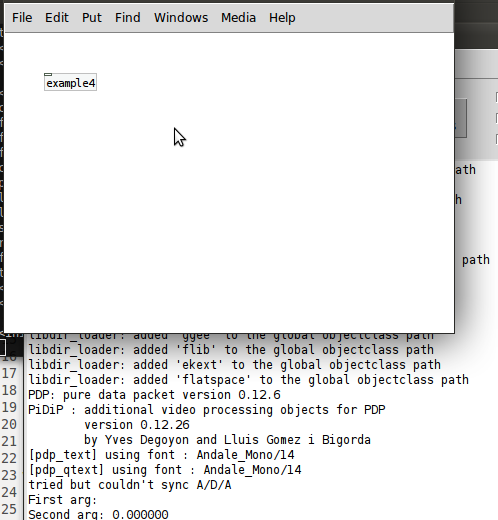
\includegraphics[width=0.7\textwidth]{example4}
\caption{Inlets passivos}
\label{fig:inlet-passivo}
\end{figure}

\section{Inlets ativos}

Um inlet ativo associa ao inlet uma função. Assim como o inlet passivo, a
criação de um inlet ativo define o tipo do átomo que o inlet receberá (veja o
exemplo 05 e o resultado na figura \ref{fig:inlet-ativo}).

\begin{lstlisting}
// all inlet-methods receive the object as their first argument.
void example5_bang(t_example5 *x) { 
  post("BANGED!");
  post("My_float value: %f",x->my_float);
}

void example5_anything(t_example5 *x, t_symbol *s, int argc, t_atom *argv){
  post("ANYTHING!");
}

void example5_setup(void) {
  example5_class = class_new(gensym("example5"),
    (t_newmethod) example5_new, // Constructor
    0, 
    sizeof (t_example5),
    CLASS_DEFAULT,
    0); // LAST argument is ALWAYS zero
  class_addbang(example5_class, example5_bang);
  class_addanything(example5_class, example5_anything);
}
\end{lstlisting}

\begin{figure}[h!]
\centering
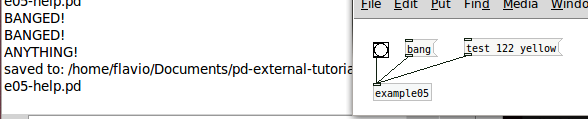
\includegraphics[width=0.7\textwidth]{example5}
\caption{Inlets ativos.}
\label{fig:inlet-ativo}
\end{figure}

Da mesma forma que ocorre com inlets passivos, cada inlet ativo é associado a
um tipo de átomo, de forma que sua definição também deve ser feita através de
funções específicas.  Abaixo, a tabela com os métodos que criam inlets ativos,
e assinaturas possíveis para funções associadas a cada tipo:

\begin{center}
\begin{tabular}{|l|l|}
\hline
método do pd para criar inlet ativo & assinatura para o método associado ao
inlet \\
\hline
\texttt{class\_addbang(t\_class *c, t\_method fn);} 	& \texttt{my\_b(t\_myt *x);} \\
\texttt{class\_addfloat(t\_class *c, t\_method fn);}	& \texttt{my\_f(t\_myt *x, t\_floatarg f);} \\
\texttt{class\_addsymbol(t\_class *c, t\_method fn);}	& \texttt{my\_s(t\_myt *x,t\_symbol *s);} \\
\texttt{class\_addpointer(t\_class *c, t\_method fn);}	& \texttt{my\_p(t\_myt *x, t\_gpointer *pt);} \\
\texttt{class\_addlist(t\_class *c, t\_method fn);}	& \texttt{my\_l(t\_myt *x, t\_symbol *s, int argc, t\_atom *argv);} \\
\texttt{class\_addanything(t\_class *c, t\_method fn);}	& \texttt{my\_a(t\_mydata *x, t\_symbol *s, int argc, t\_atom *argv);} \\
\hline
\end{tabular}
\end{center}

\section{Tratamento de mensagens no primeiro inlet}

É possível associar átomos a métodos e executar métodos diferentes dependendo
do conteúdo das mensagens recebidas pelo primeiro inlet. Isto é feito através da
função \texttt{add\_method()} veja o exemplo 08).

\begin{lstlisting}
// Constructor of the class
void * example8_new(void) {
  t_example8 *x = (t_example8 *) pd_new(example8_class);
  // create an inlet that calls the method "example8_alfa"
  inlet_new(&x->x_obj, &x->x_obj.ob_pd, gensym("float"), gensym("alfa"));
  return (void *) x;
}

void example8_start(t_example8 *x){
  post("START / BANG");
}

void example8_open(t_example8 *x, t_symbol *s){
  post("open %s",s->s_name);
}


void example8_alfa(t_example8 *x, t_floatarg f){
  post("ALFA VALUE %f",f);
}

void example8_setup(void) {
  example8_class = class_new(gensym("example8"),
    (t_newmethod) example8_new, // Constructor
    (t_method) example8_destroy, // Destructor
    sizeof (t_example8),
    CLASS_DEFAULT,
    0); // LAST argument is ALWAYS zero
  // All these messages will be received by the first left inlet
  class_addmethod(example8_class, (t_method) example8_start, 
    gensym("start"), 0); // two messages, the same function
  class_addmethod(example8_class, (t_method) example8_start, 
    gensym("bang"),  0); // may be "start" or "bang" messages
  class_addmethod(example8_class, (t_method) example8_open,  
    gensym("open"),  A_DEFSYMBOL,0);
  // These messages will be associated with inlet 2
  class_addmethod(example8_class, (t_method) example8_alfa,  
    gensym("alfa"), A_DEFFLOAT,0); 
}
\end{lstlisting}

Desta forma não precisamos tratar a mensagem que o inlet recebe mas definí-las
de antemão e criar funções que mapeiem a mensagem recebida. Veja a figura
\ref{fig:mais-inlets}.

\begin{figure}[h!]
\centering
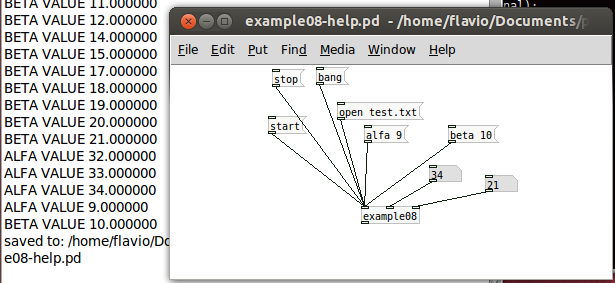
\includegraphics[width=0.7\textwidth]{example8}
\caption{Mais inlets.}
\label{fig:mais-inlets}
\end{figure}

O método \texttt{inlet\_new()} pode ser utilizado para criar inlets genéricos
que terão com métodos associados através de símbolos de mensagens:

\begin{lstlisting}
t_inlet *inlet_new(t_object *owner, t_pd *dest,
      t_symbol *s1, t_symbol *s2);
\end{lstlisting}

\section{Oulets}

Depois de termos tratado as formas de entrada de dados através de inlets do
Pure Data, chegou a hora de falarmos das saídas. A saída de dados dos objetos
do Pure Data é feita por meio de outlets (veja o exemplo 06).

\begin{lstlisting}
typedef struct _example6 {
  t_object x_obj;
  t_outlet *my_outlet; // Defines an outlet
} t_example6;

// The BANG method, first inlet
void example6_bang(t_example6 *x) {
  post("BANGED!");
  outlet_bang(x->my_outlet); // Bang my outlet
}

// Constructor of the class
void * example6_new(t_symbol * arg1, t_floatarg arg2) {
  t_example6 *x = (t_example6 *) pd_new(example6_class);
  x->my_outlet = outlet_new(&x->x_obj, gensym("bang"));
  return (void *) x;
}

void example6_setup(void) {
    example6_class = class_new(gensym("example6"),
      (t_newmethod) example6_new, // Constructor
      0, 
      sizeof (t_example6),
      CLASS_DEFAULT,
      A_DEFFLOAT, // First Constructor parameter
      A_DEFSYMBOL, // Second Consctructo parameter
      0); // LAST argument is ALWAYS zero
    class_addbang(example6_class, example6_bang);
}
\end{lstlisting}

Um outlet deve ser definido na estrutura do objeto e instanciado pela função
\texttt{outlet\_new()}, definindo também o tipo do átomo associado. No caso
deste exemplo, o outlet é do tipo \texttt{bang} e dispara um bang toda vez que
recebe um bang (veja a figura \ref{fig:outlet-bang}).

\begin{figure}[h!]
\centering
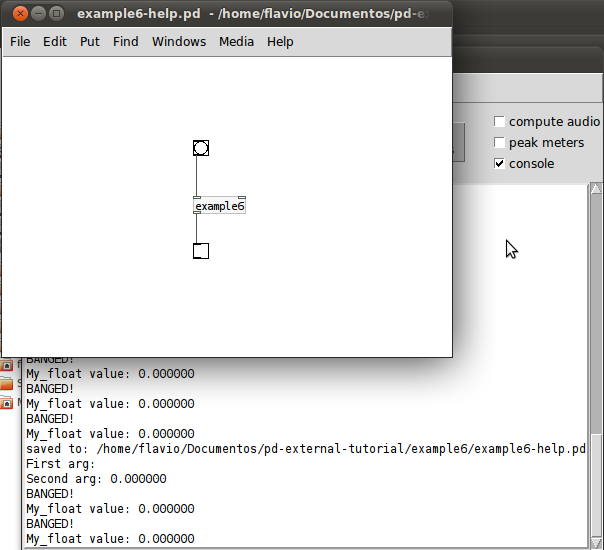
\includegraphics[width=0.7\textwidth]{example6}
\caption{Um external bem útil que recebe um bang e envia um bang.}
\label{fig:outlet-bang}
\end{figure}

\todo{Tem um tipo de inlet/outlet que utiliza um sistema de proxy para que os
mesmos possam ser definidos on the fly. Nunca usei mas acho que seria legal abordar.
 Ele baseia-se em definir um método em outro objeto (o proxy) e associar
este novo inlet ao proxy. Assim podemos instanciar vários proxys e tratar vários
inlets passivos, por exemplo.}
